\documentclass[a4paper]{article}
\usepackage{graphicx}

\begin{document}
\title{Buffalo}
\author{}
\date{}

\maketitle

Your village is under attack! The buffalo are going to over-run the village unless you can stop them getting over the river.

\section*{Aim}
The aim of this game is to stop the buffalo crossing the river. If one buffalo crosses the river at the top, the indian loses. The indian wins when the buffalo are all blocked by dogs or the indian.

\section*{How to play}
\begin{figure}[htb]
	\begin{center}
		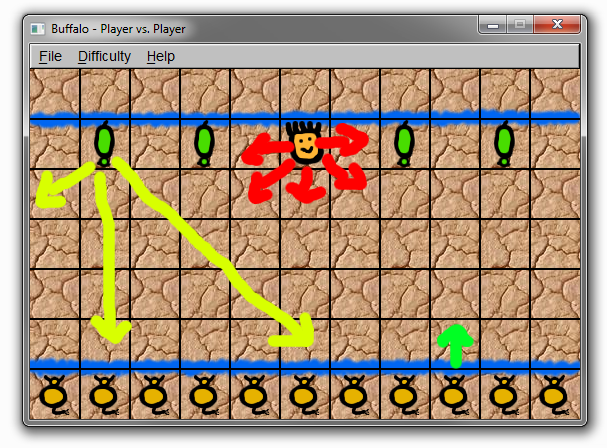
\includegraphics[width=\linewidth]{figureinstructins.png}
	\end{center}
	\caption{A new player vs.\ player game indicating the possible moves of three pieces}
	\label{fig:instructins}
\end{figure}
The pieces in this game move similar to chess (see figure \ref{fig:instructins}).
\begin{description}
	\item[Indian] The indian can move like a king and is the only piece capable of taking a buffalo.
	\item[Dog] A dog can move like a queen and are useful for blocking buffalo
	\item[Buffalo] Buffalo can only move one space forward per turn. Buffalo go first.
\end{description}
The indian player has 4 dogs to aid him. Indians move like kings and are the only piece that can take buffalo. Dogs can move like queens. Buffalo move like pawns. Dogs and Buffalo cannot move on top of each other.

\section*{Modes of Play}
There game defaults to Player vs.\ CPU (easy) with the computer controlling the buffalo. One can set the CPU difficulty level or start a new game of Player vs.\ Player.

\section*{Good Luck!}
This game was made by Nathanael Farley based on a board game called `Buffalo' or `Trespass'. Happy protecting!
\end{document}
